\title{Practical study of AnyDSL GPGPU program partial evaluator}
\titlerunning{Practical study of AnyDSL GPGPU program partial evaluator}

\author{Aleksey Tyurin}
\authorrunning{Aleksey Tyurin}

\tocauthor{Aleksey Tyurin}
\institute{St Petersburg State University\\
	\email{aleksey.tyurinspb@gmail.com}}

\graphicspath{{Tyurin/}}

\newtheorem{mytheorem}{Theorem}
\newtheorem{mydef}{Definition}
\renewcommand{\abstractname}{Abstract}
\renewcommand*{\proofname}{Proof}
\renewcommand*{\figurename}{Figure}
\renewcommand*{\tablename}{Table}
\renewcommand*{\refname}{References}


\maketitle

\begin{abstract}
	The optimization of GPGPU programs has steadily received close attention 
	in the research community since applications ought to be more effective,
	 less memory consuming, and easier to program.
	  Partial evaluation in turn is a tool that could automatically bring performance leveraging the static nature of the application inputs.
	   This work aims to combine partial evaluation and GPGPU programs to make the latter more memory efficient.
It analyses whether any performance gain could be achieved via
 data access embedding achieved by partial evaluation and identifies GPU-specific details that affect the effectiveness of partial evaluation.
\end{abstract}


\section*{Introduction}\label{sec:introduction}
In the era of big data and high load computations, graphical processing units
 (GPUs) are used extensively for data processing. 
 There have even been designed embedded devices with the support of GPUs
  for general purpose computations, like image recognition on mobile robots~\cite{NVJETSON}.
In practice many GPU-based applications tend to be bandwidth bound, meaning
 that data allocation and access are the main bottlenecks, thus memory optimizations
  appear to be in a prevailing significance and are addressed in a huge amount of research.

While the problem of available GPU memory could be tackled with sophisticated memory pooling techniques
 through memory swapping and sharing~\cite{zhang2019efficient},
  memory architecture of a GPU often requires more sophisticated optimizations.
   Given that a typical GPU incorporates several memory types, each having different
    capacity and throughput, a few memory management automation techniques have been introduced. They could leverage more effective memory spaces to handle register spilling and systematically consider the performance benefit achievable through a specific allocation of shared memory to save global memory transactions~\cite{AutomaticSharedMem,RegisterSpilling}. Further, the diversity of memory types imposes that each memory access should satisfy memory type specific patterns, to be most effective. Under the non-fulfillment of these patterns the data throughput of an application is aggravated due to the increase in the number of required memory transactions. Considering the following typical scenario of a GPU-accelerated application, another runtime memory optimization could be proposed.

 To facilitate the data processing a GPU routine is executed by multiple threads simultaneously with different pieces of data, often exceeding the maximal number of threads
  that could be executed simultaneously resulting in blocks of threads being executed iteratively.
 Being that the input data often exceeds the available GPU memory, the routine could not be applied at once, 
 and there is a need to split the data into chunks and process them iteratively 
 by the routine.
 It happens that some relatively small properties within a processing routine are maintained between the iterations
  and could be considered static in that sense.
 For example, if the application is a GPU-accelerated data processing engine that allows one to write queries to data and typically these queries remain small if compared to data and take significant execution time, the query, once specified by the user, can be used as a static, i.e. already known and constant, data for the query execution kernel runtime optimization since it remains unchanged during the host code execution.
 This observation allows to apply a \textit{partial evaluation} technique to optimize such routines in runtime.

\textit{Partial evaluation} or program \textit{specialization}~\cite{Jones1993,PartialEvalPaper} is a program
 transformation and optimization technique that optimizes a given program with
  respect to statically known inputs, producing another program which,
   if given only the remaining dynamic inputs, will produce the same results
    as initial one would have produced, given both inputs.
Basically, a partial evaluator performs an aggressive unfolding/unrolling, 
inlining, and constant propagation.  
The application of partial evaluation at runtime has 
recently shown a significant performance improvement of query execution for CPU-based
 database querying~\cite{LLVMmix}. 

Regarding memory optimizations of GPU kernels, partial evaluation is 
able to embed static data memory accesses into the code, i.e. place it directly 
into registers, once a kernel is properly written, which could result in a better
 performance compared to non-embedded access since memory transactions would be replaced 
 by accesses to the instruction cache. Thus, the aim of this work is to provide 
 an empirical evaluation of an existing partial evaluator AnyDSL~\cite{LeiBa} 
 that is capable of producing CUDA~\footnote{Programming and hardware model by NVIDIA.} code for NVIDIA GPUs
  to investigate the effects that appear after partially evaluating GPU applications,
   and what aspects of GPU architecture affect the desired result and 
   whether any significant performance improvements could be achieved at all.
   More specifically, the work performs the evaluation on string matching and convolutional filtering scenarios, providing some relevant CUDA assembly examples to ground the effects being observed.

\section{Обзор схожих работ}

\paragraph{Подтипирование между закрытыми типами}
Существует ряд из исследовательских работ о номинальном подтипировании с вариантностью между закрытыми типами. В одной из последних таких работ была показана Тьюринг-полнота подтипирования в \java{}~\cite{grigore2017java}. C++ шаблоны также Тьюринг-полны~\cite{veldhuizen2003c++}. Системы типов Scala \cite{odersky2016scaling}, OCaml \cite{lillibridge1997translucent, rossberg1999undecidability} и Haskell с расширениями~\cite{sulzmann2007understanding} неразрешимы. Напротив, подтипирование в \dotnet{} разрешимо~\cite{emir2006variance,kennedy2006decidability}. Упомянутые статьи формализуют и исследуют \emph{проверку типов} в некоторых языках программирования. Мы же исследуем подтипирование учитывая открытые типы, основываясь на результатах о подтипировании между закрытыми типами.

\paragraph{Выполнимость ограничений}
Одной из последних близких нам работ является~\cite{sherman2015deciding}. В ней, действуя в соответствии с  теми же целями, сводят проблему выполнимости для частично упорядоченных множеств, основанных на типах, к проблеме выполнимости в языке первого порядка, и предлагают использовать SMT-решатели для решения ограничений. В отличие от нашей работы, рассматривается только номинальный фрагмент системы типов \java{} без обобщённых типов.

Проблема выполнимости ограничений, и её вычислительная сложность для более общих (в сравнении с ~\cite{sherman2015deciding}) фрагментов системы типов исследуется в ~\cite{pratt1996satisfiability, frey1997satisfying, kuncak2003structural, niehren2005complexity}. Эти работы исследуют ограничения на конечные и рекурсивные типы, структурное и не структурное подтипрование и типовые конструкторы с ковариантными и контравариантными типовыми параметрами. Наша работа изучает более общую проблему.

В~\cite{su2002first} показывается неразрешимость задачи выполнимости ограничений для не структурного подтипирования. Этот результат влечёт неразрешимость \subtypesat{}, но для его доказательства используется значительно больший фрагмент логики первого порядка (например, формулы с кванторами всеобщности). Наше доказательство использует только бескванторные конъюнкции положительных атомов, однако, оно также использует особенности номинального подтипирования с вариантностью, которых нет в не структурном подтипировании.

\section{Experimental setup}
In this section, the scheme of runtime partial evaluation is presented as well as the evaluation configuration.

\subsection{Runtime partial evaluation}

\begin{figure}
    \centering
    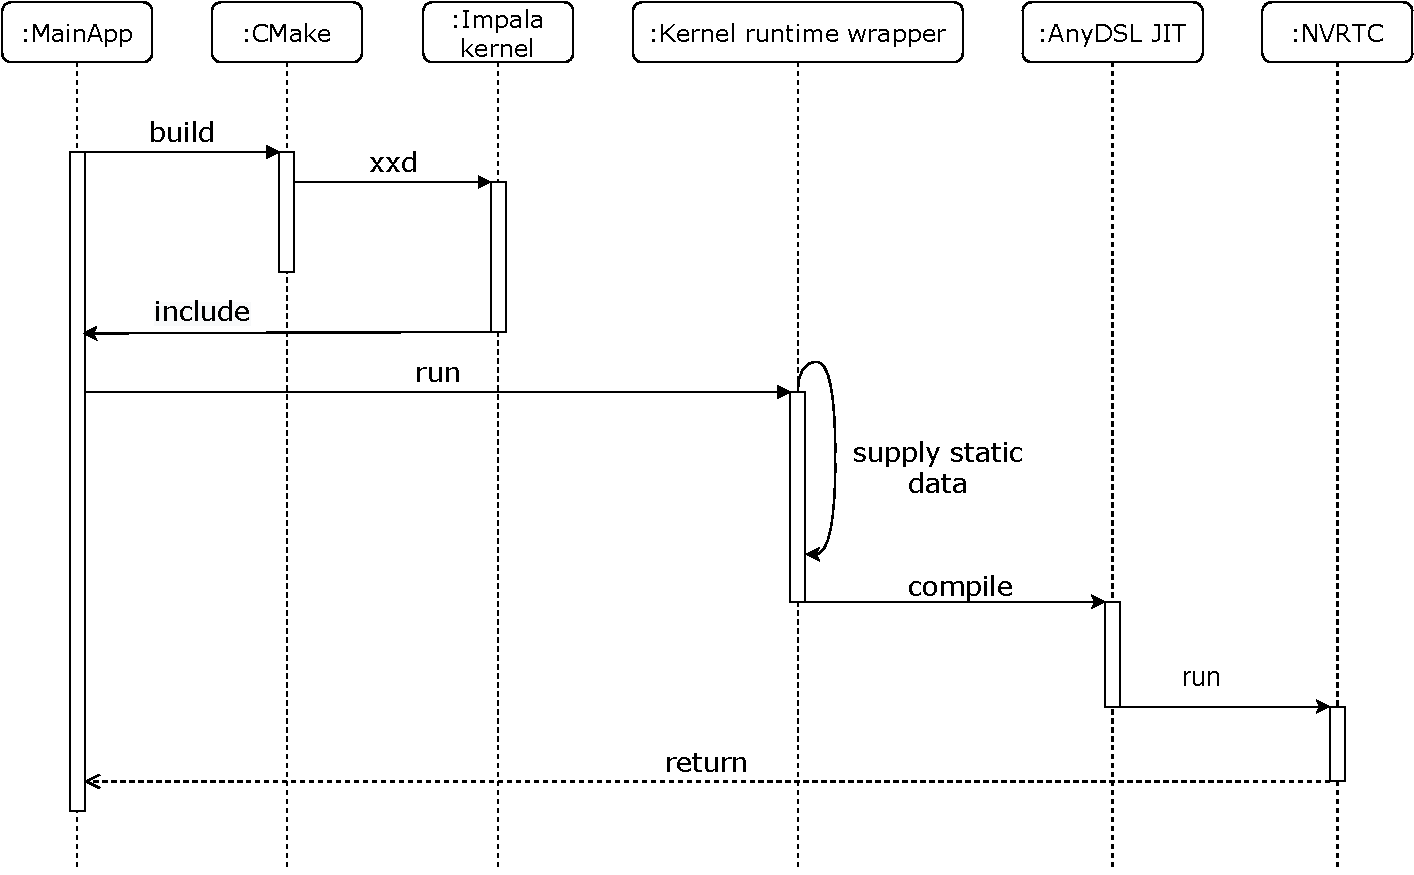
\includegraphics[width=\linewidth]{figures/SeqDiagram.pdf}
    \caption{Runtime partial evaluation diagram}
    \label{fig:seq_pe}
\end{figure}

In practice, it is infeasible to compile a new kernel for each static input 
value, which is often known in runtime. Thus the partial evaluation of the 
kernel should be performed in runtime as well as the kernel compilation to 
a specific GPU target.
Each specialized benchmark scenario corresponds to the sequence in 
figure~\ref{fig:seq_pe}. The device kernel in Impala is included in the 
target application using \lstinline{xxd} tool during the compilation. 
When static data becomes known at runtime, the kernel wrapper is constructed, 
that supplies the static data to the included kernel, 
creating partially applied kernel. Then AnyDSL JIT compiler is invoked, 
which specializes the kernel according to the annotations provided, 
and static arguments supplied, generating CUDA C code, which is then passed 
to NVRTC\,\footnote{\url{https://docs.nvidia.com/cuda/nvrtc/index.html} (last accessed date: 30.05.2020)} 
and got eventually compiled to GPU assembly and invoked.

The evaluation aim is to show whether a device kernel could benefit from data 
embedding performed by partial evaluation and possible reduction of 
static computations. For the data to be embedded, the accesses should 
be static, which is a standard scenario for constant memory to be used to store such data, 
thus constant memory is a baseline in several scenarios. 
Further, only the execution time of a device kernel should be measured, 
since, for example, overhead for partial evaluation and JIT compilation 
for a device could be hidden by GPU data transferring or other workarounds.

Since NVRTC is internal to AnyDSL framework, 
the benchmarking results could be obtained via 
nvprof\,\footnote{\url{https://docs.nvidia.com/cuda/profiler-users-guide/index.html} \\ (last accessed date: 30.05.2020)} 
or by utilizing a specially recompiled version of the framework 
runtime with CUDA events. 
The latter option is used since it allows to perform warm-up runs of the kernel 
to make the benchmarking more reliable. The whole system is implemented in C++ and Python, 
and enclosed into a Docker container with the datasets indexed in Git LFS\footnote{\url{https://git-lfs.github.com/} (last accessed date: 30.05.2020)}
 for benchmarks to be easily built and run on any system with NVIDIA GPU\,\footnote{\url{https://github.com/Tiltedprogrammer/spec} (last accessed date: 30.05.2020)}. 
 The following GPGPU scenarios have been implemented, which are fit under the described in~\ref{PEsurvey} pipeline.
\begin{itemize}
    \item Na\'ive single substring matching.
    \item Na\'ive multiple substring matching.
    \item Aho--Corasick matching.
    \item 2-D convolution filter.
\end{itemize}
The following system has been used to run the benchmarks: 
Ubuntu 18.04 with CUDA Toolkit 10.2. hosted in Google Cloud 
bundled with 4 cores of Intel Xeon and NVIDIA Tesla T4 GPU.

\section{Evaluation}
In this section, the implementation details of the benchmarks are provided, 
as well as the selected datasets, and GPU architecture details that affect 
the result. A general workflow of analyzing GPU-code is also could be seen 
in this section. 

\subsection{String matching}
GPU-accelerated string matching frequently appears in GPU-based data\-bases, 
file carving~\cite{DataCarving,GPU-carving} that stands for extracting 
files from raw data in a field of cyber forensics, and intrusion 
detection~\cite{GPU-IDS}. Thus such a problem has a huge practical 
interest. Substrings could be considered static and subjected to 
partial evaluation.

\subsubsection{Na\`ive single substring matching}\label{naive-single}
Na\`ive algorithm operates on a \emph{subject} string and a \emph{pattern}, 
iteratively comparing each symbol of the pattern with the 
symbols of each substring of the subject string of size equal to the size 
of the pattern. The algorithm is inherently data-parallel: such substrings 
could be traversed separately, each in their thread. Further, such a traversal 
provides a rather optimal global memory access pattern, since adjacent 
threads would access addresses of adjacent substrings. There exist an opportunity 
for optimization, since at one moment all threads in a warp access the same symbol 
of the pattern (and distinct symbols of the subject string), thus the pattern could 
be placed in constant memory to speed up the performance.

%<3 pushishku <3
 
There is a \emph{KMP} test for optimizers like partial evaluator, 
intended to check whether they correctly reduce static computations. 
Partial evaluation is able to reduce a na\`ive single substring matching, 
though properly rewritten, to something very like Knuth--Morris--Pratt algorithm~\cite{KMP-Danvy}, 
which uses a prefix function to recover from a mismatch, thus being linear with 
respect to the subject string.
When a mismatch occurs, it is known that all previous symbols of the pattern 
match the ones of the substring of the subject string up to the point of mismatch. 
In order to simulate a prefix function at the mismatch point, the pattern could be 
matched against itself up to this point, searching for the largest prefix being a 
suffix as well.
Since the pattern is static and matched against itself, this computation is fully static 
and could be performed at specialization time.
Porting this approach to GPU and Impala, and applying partial evaluation 
at runtime indeed produces a KMP-like program\footnote{\url{https://github.com/Tiltedprogrammer/spec/blob/master/kmp.dump}\\ (last accessed date: 30.05.2020)}. 
Thus, making the used partial evaluator sound in a sense. The KMP algorithm itself is hard to partially evaluate since the already matched piece of the pattern 
that drives the search through the backtracking table is fully dynamic.

However, such an approach is far less data parallel as well as KMP. The subject 
string should be divided into interleaved chunks, each assigned to a different 
thread. Such parallelization has a far worse access pattern since each 
thread accesses strided addresses of the subject string. 
However, in practice, such an access pattern occurs when the search is performed 
across different subject strings, where each thread operates on a 
specific string\footnote{\url{https://github.com/NVIDIA/nvstrings} \\(last accessed date: 30.05.2020)}

A na\`ive single substring matching could be also specialized by simply unrolling 
the traversal, that does not hurt the parallelization. 
The evaluation of these approaches is presented in figure~\ref{fig:kmp_test}.

\begin{figure}
    \centering
    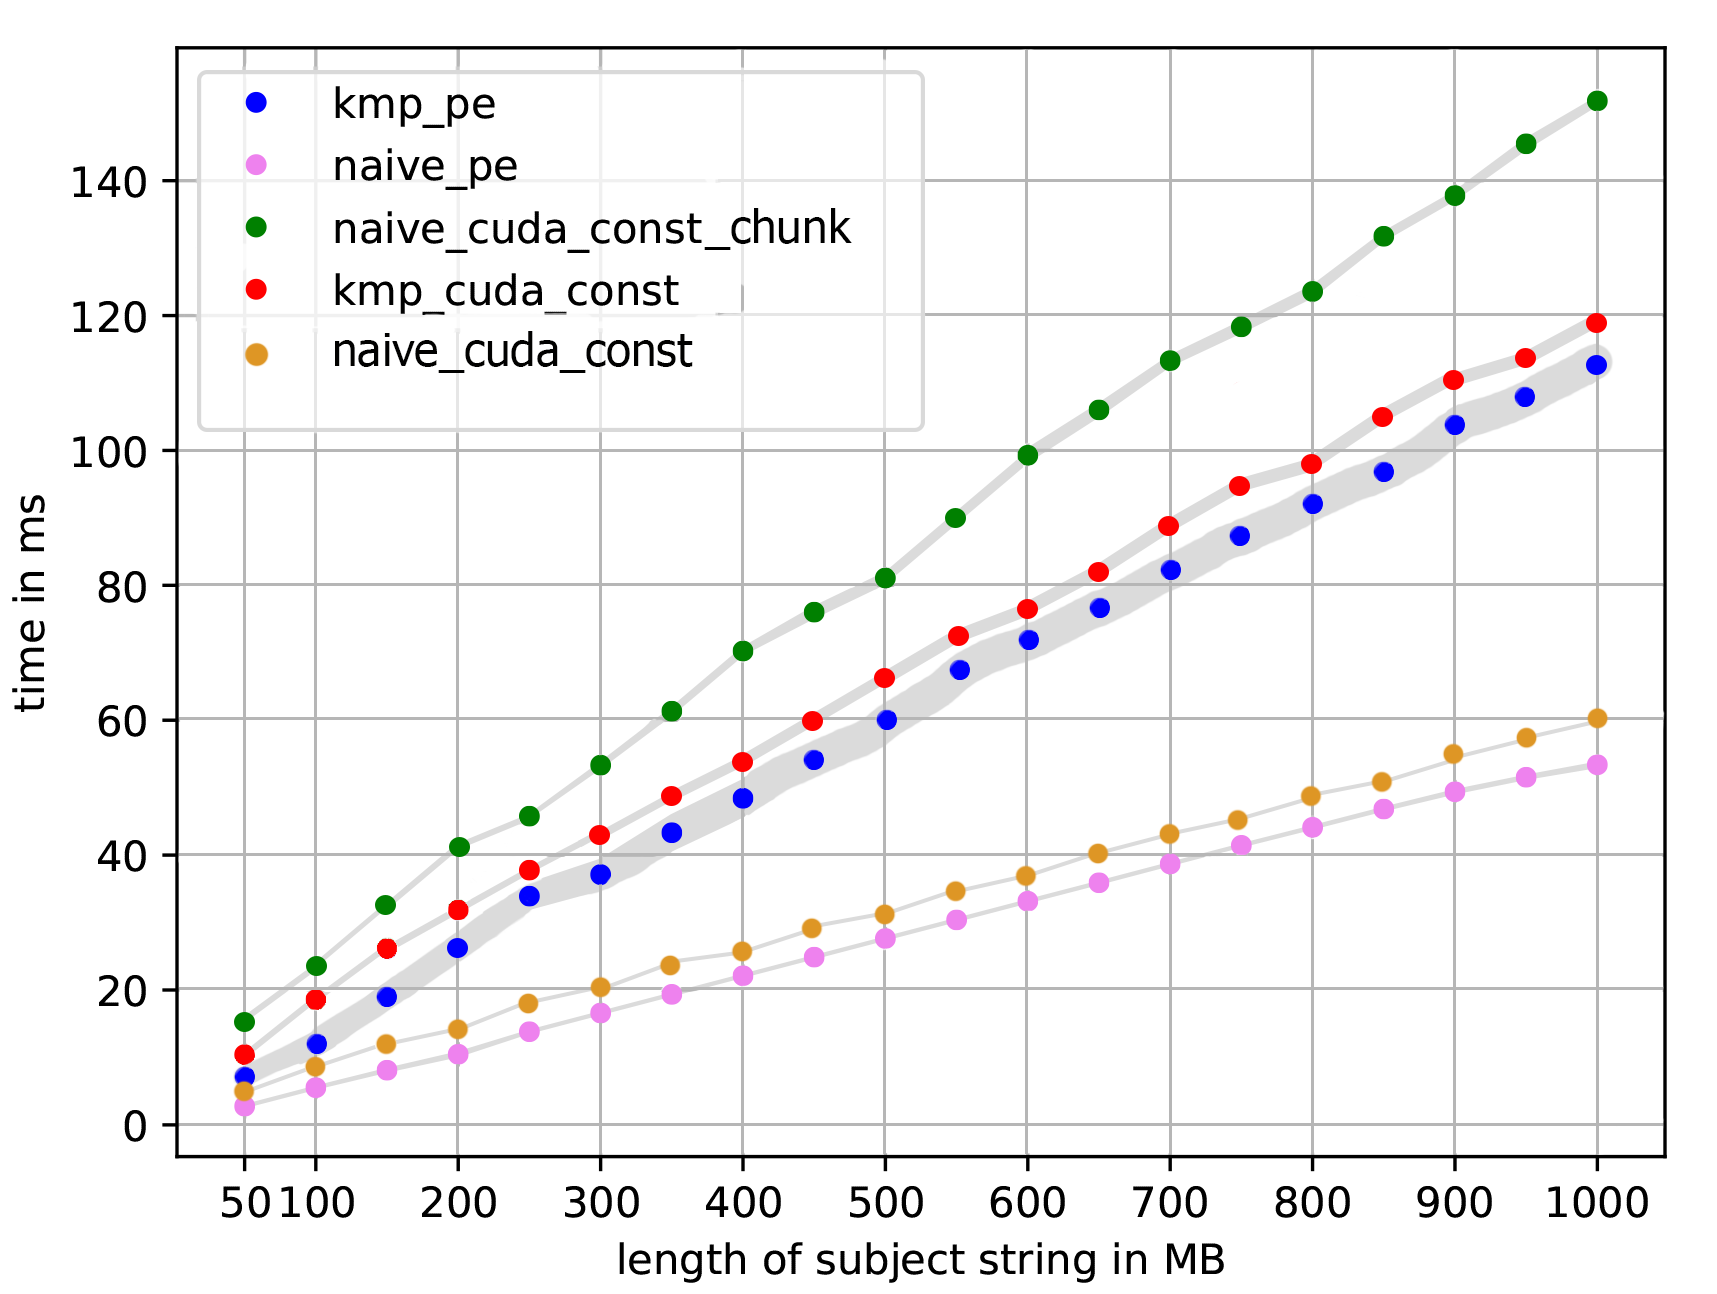
\includegraphics[width=0.85\linewidth]{figures/KMP_TEST.png}
    \caption{Na\`ive single substring matching}
    \label{fig:kmp_test}
\end{figure}

The current recursive implementation of the partial evaluator does not 
handle well the KMP test with patterns of more than 16 bytes in length. 
Thus, for the evaluation, a set of uniformly randomized 50 patterns\footnote{Enough for the divergence not to affect deviation so much.} 
from two-characters alphabet has been taken, satisfying that restriction. The subject string has been also randomly generated from the same alphabet. The standard deviation is shown in gray regions.
The KMP algorithm obtained by partial evaluation (\emph{kmp\_pe}), KMP algorithm implemented with CUDA, utilizing constant memory to store the backtrack table and the pattern (\emph{kmp\_cuda\_const}), 
na\`ive algorithm in CUDA with chunk-based parallelization (\emph{naive\_cuda\_const}), naive\`ive algorithm in CUDA with char-based parallelization and its partially evaluated version, that embeds the 
pattern into the code through unrolling the traversal, are compared. The figure grounds the success of the KMP test and shows that data embedding does not give any significant improvements: the difference 
between embedded and not embedded versions are mainly due to the reduced amount of address computations and loop overhead. The char-based parallel version is at the bottom due to a better memory access policy.

\subsubsection{Data embedding}\label{data_embedding}
Partial evaluation for the scenario above performed the transformation 
similar to the one in listing~\ref{code:kmp_spec}. While the load/store 
speed comparison for memory spaces is well described~\cite{TeslaT4Bench}, 
e.g. non-conflicting constant load is faster than L1 cache hit, the behavior 
of such embedded data is unspecified, but could be deduced as follows.
Embedded values could either inhabit a register, when e.g. \mintinline{C}{MOV R1 0x62}
 instruction occurs or be immediate-value parameters of the instructions. 
  The mini benchmark from listing~\ref{code:mem_bench} shows that embedded values are accessed through instruction cache by measuring the
   number of cycles required to perform an addition operation
   \mintinline{LLVM}{add.u32} with one of the arguments passed via embedded value or 
   via constant memory, lines 9 and 13. Given such a benchmark, the version with the value 
   embedded performs 10 times faster: 42 cycles versus 430 on a constant cache miss. If the constant 
   cache is firstly warmed up, the latency becomes 42 cycles and is the same for both instructions. 
   Thus, embedded values are more likely to be accessed via instruction memory, since 
   the instructions are prefetched and would outperform constant memory access under cache misses. 
   
   \begin{listing}
    \begin{pyglist}[language=C, caption=Memory benchmark,label=code:mem_bench]
__constant__ int mini_array [2];
    
__global__ void dummy_kernel(int* dst,int* clocks){
        
    int i;
    int start,stop;
        
    asm volatile("mov.u32 %0, %%clock;": "=r"(start) :: "memory");
    asm volatile(
                "add.u32 %0, %1, 12;\n\t"
                :"=r"(i) :"r"(i): "memory");
    // vs
    asm volatile(
                "add.u32 %0, %1,%2;\n\t"
                :"=r"(i) :"r"(i),"r"(mini_array[0]: "memory");
    asm volatile("mov.u32 %0, %%clock;": "=r"(stop) :: "memory");
    }
    \end{pyglist}
    \end{listing}

   Notably, when embedding, a partial evaluator is able to generate a more effective instruction, e.g. 
   shift instead of division, which takes more than 10 instructions on GPU, 
   while shift requires only one.

\begin{listing}
\begin{pyglist}[language=C,caption=KMP partial evaluation,label=code:kmp_spec]
    //kmp_cuda_const
LDC R0, c[0x3][R0] //load pattern's character
    //...//
    
LDG R12, [R2] //load subject's character
ISETP.NE.AND P0, R0, R12 // compares
    //..//

LDC R4, c[0x3][R2] // in case of mismatch go to backtrack position

    //kmp_pe
LDG R12, [R2] //load subject's character from global memory
    //    ...
ISETP.NE.AND P0, R12, 0x61 // pattern's char is put into the instruction
\end{pyglist}
\end{listing}

\subsubsection{Na\`ive multiple substring matching}\label{nmsm}

\begin{figure}
    \centering
    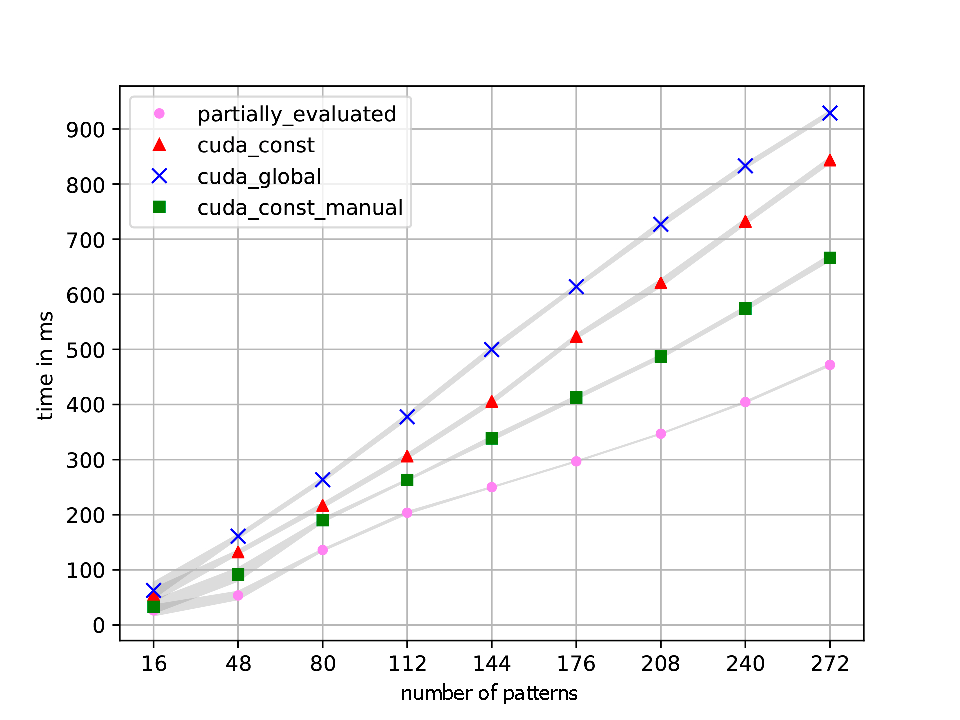
\includegraphics[width=0.85\linewidth]{figures/PredDefendNaiveSearch.pdf}
    \caption{Na\`ive multiple substring matching}
    \label{fig:naive_multy}
\end{figure}

The core of the algorithm is the same as the one of~\ref{naive-single} with the addition that a set of patterns is traversed against the substring. Since a set of patterns is traversed, their sizes are needed to be accessed, in order to be able to determine the border between the patterns. Constant memory could be utilized to store the sizes and the patterns, since threads of a warp access the same size and the same symbol of the pattern. Partially evaluating the algorithm with respect to the patterns, allows to fully reduce all the memory accesses to the sizes, which are numerous when the subject string is huge. Partial evaluation is achieved through loop unrolling for the sizes and the patterns. The results of this benchmark are presented in figure~\ref{fig:naive_multy}.

The dataset under use is from the intrusion detection area, which is common for multiple pattern matching problems~\cite{Aho-Corasick}. 
The subject string is 500MB \emph{tcpdump} from \emph{Botnet} 
dataset~\cite{Ring_2019}. The patterns are extracted from 
\emph{Snort V3}\footnote{\url{https://www.snort.org/downloads} (last accessed date: 30.05.2020)} 
rules, which are the patterns containing malicious traffic. 
The same set of patterns has been run over 30 times taking the average. 
The gray area represents the standard deviation.

\emph{Cuda\_global} is the implementation with global memory for storing the sizes 
and the patterns, while \emph{cuda\_const} uses constant memory for this. 
As it could be seen, the partially evaluated version is at the very 
bottom being 2x faster than the version with constant memory. 
\emph{cuda\_const\_manual} is the implementation, where all size accesses 
have been reduced manually, using a CUDA JIT 
compiler\footnote{\url{https://github.com/NVIDIA/jitify} \\(last accessed date: 30.05.2020)}. 
It is slower than the partially evaluated version due to the fact that all CUDA instruction arguments should be at least 4 B in size.
As shown in listing~\ref{code:vs}, access and later use of 1 B size values requires their extension to 4 B word, while 
the immidiate-value parameters require no such extension. However, partial evaluation does not save memory since the 
code populated with embed values grows due to unrolling.

\begin{listing}
    \begin{pyglist}[language=C,caption=Cuda\_const\_manual vs partially\_evaluated,label=code:vs]
        //Cuda_const_manual
    
IMAD.MOV.U32 R8, RZ, RZ, R4 
ULDC.64 UR4, c[0x0][0x160]
IMAD.MOV.U32 R9, RZ, RZ, R3
LDG.E.U8.SYS R8, [R8.64+UR4+0x1] // load subject's character
ULDC.U8 UR4, c[0x3][0x1] //load pattern's character
ULOP UR4, UR4, 0xff, URZ, 0xc0
IMAD.U32 R11, RZ, RZ, UR4
PRMT R11, R11, 0x9910,RZ
PRMT R12, R8, 0x9910,RZ
ISETP.NE.AND P0, PT, R12, R11, PT //compare

    //partially_evaluated

IMAD.MOV.U32 R6, RZ, RZ, R2 
ULDC.64 UR6, c[0x0][0x160] 
IMAD.MOV U32 R7, RZ, RZ, R5 
LDG.E.U8.SYS R6, [R6.64 + UR6+0x1] // load subject's character
PRMT R8, R6, 0x9910, RZ
ISETP.NE.AND P0, PT, R8, 0x42, PT //compare
    
    \end{pyglist}
    \end{listing}

It could be tempting to embed data of size exceeding a constant memory pool 
of 64 KB into code, provided that such access could be even faster. But 
firstly, CUDA limits the maximum number of instructions that could be put into a module by 512 million, and, secondly, 
compilation time begins to matter for relatively huge embedded data, 
e.g. 272 patterns are about 5KB in size and compilation took several minutes.


\subsubsection{Aho-Corasick matching}
Aho-Corasick is a time efficient algorithm for 
multiple string pattern matching~\cite{Aho-Corasick} 
and based on suffix tree and a failure transition table. 
However, a failure transition table becomes redundant by switching 
to GPU, since a simple suffix tree traversal per thread for each 
position in the subject string appear to be more efficient~\cite{PFAC}. 
The parallel Aho-Corasick first construct a transition table where final 
states have numbers less than the starting state, to reduce memory accesses 
for checking whether the state is final or not. The table is stored in 
global memory and each thread traverses the table taking a subject 
string character from shared memory. The benchmark and the implemented 
algorithms are presented in figure~\ref{fig:my_corasick}. The dataset used is 
the same as in~\ref{nmsm}. \emph{Cuda\_corasick\_lib} is the implementation 
of this algorithm\footnote{\url{https://github.com/pfac-lib/PFAC} \\
 (last accessed date: 30.05.2020)} taken from~\cite{PFAC}. The transition table is often sparse and could be embedded into the code during partial evaluation using static binding of dynamic variables~\cite{Jones1993} avoiding empty entries, \emph{corasick\_pe} is the implementation of this approach. \emph{Naive\_pe} is the algorithm from~\ref{nmsm} utilizing shared memory. \emph{Cuda\_corasick\_pe} is the implementation, where a pattern set specific interpreter for the transition table is generated. The interpreter represents a sequence of code-embedded conditional statements to traverse the suffix tree.


\begin{figure}[h!]
    \centering
    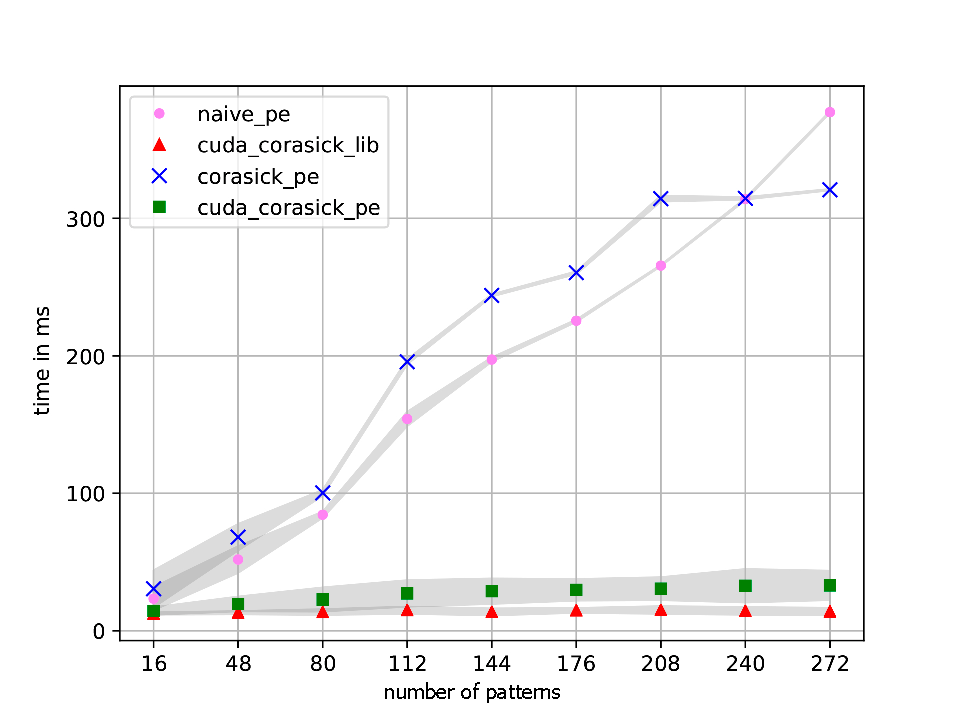
\includegraphics[width=\linewidth]{figures/PredDefendNaiveSearchorasick(eng).pdf}
    \caption{Aho-Corasick matching}
    \label{fig:my_corasick}
\end{figure}

Static binding is a traversal of statically known possible values of a dynamic 
parameter in a bunch of condition statements. In this case, such an approach 
induces more thread divergence, e.g. 6 times if compared to \emph{cuda\_corasick\_lib}, 
which drastically decreases the performance of a GPU application. 
The interpreter approach has better divergence behavior but still diverges 
twice as much as \emph{cuda\_corasick\_lib}. So, given that global memory access 
latency even on L1 cache hit is more than the one for embedded data, 
the static binding approach that could work well on a CPU has a poor 
performance when a GPU is used, and even if interpretative implementation is 
near, such an embedding also does not provide any performance benefit.

\subsection{Convolutional filtering}

\begin{figure}[h!]
    \centering
    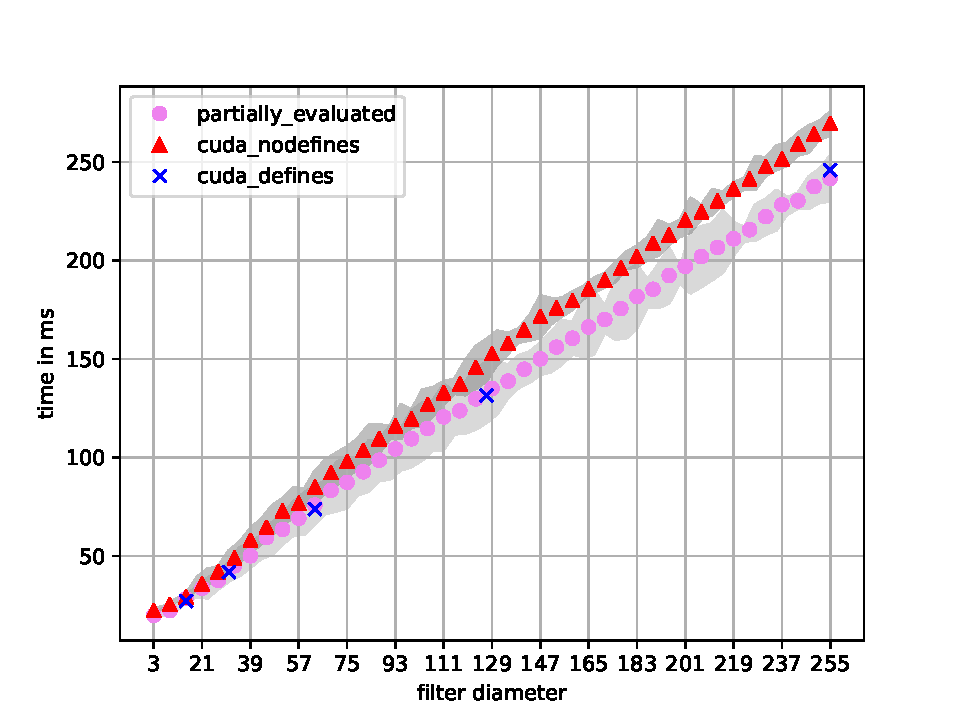
\includegraphics[width=\linewidth]{figures/separable_convolution_diploma.pdf}
    \caption{Separable convolution}
    \label{fig:convolution}
\end{figure}

Convolutional filtering is a matrix dot product frequently used in image processing~\cite{chetlur2014cudnn}. Basically, there are a huge subject matrix and a small filter matrix, and each submatrix of the subject matrix is dot producted with the filter matrix.
Since the filter is small and is static, the convolution operation could be partially evaluated with respect to the filter.
A partial evaluation for a 2-D separable\footnote{1-D filter could be applied first to rows and then to columns.} convolutional filtering has been performed in~\cite{OnlinePe}, targeting different hardware, however, the described filter is a rewritten modification of the reference filter, thus the obtained speed-up is not achieved by means of partial evaluator solely, and is used to demonstrate the facilities of the Impala language.

\subsubsection{Separable convolution}

A separable convolutional filter has been implemented in CUDA and 
Impala~\cite{CudaConv}. It operates on a 2-D array in global memory with 
threads organized in $32 x 16$ blocks, where each thread convolves 8 elements. 
Shared memory is utilized to store the big area for convolution with a block 
and the required borders. Since the filter is read-only and accessed equally 
by all the threads, it is stored in constant memory. Elements that fall away 
the borders of the 2-D subject array are assigned zeroes. 
There are two device kernels to perform a convolution: one convolves the rows 
and the other convolves the columns with the shared memory padded enough to 
not cause bank conflicts when accessing column elements.

\begin{listing}
    
\begin{pyglist}[language=C,label=code:conv,caption=Convolution partial evaluation]
//cuda_defines
LDS.U R16, [R2 + 0x38] //load from shared
FFMA R17, R10, c[0x3][0x1dc] R17 //float multiply add

//partially_evaluated
LDS.U R16, [R2 + 0x38] //load from shared
FFMA R17, R10, 42 R17 //float multiply add

\end{pyglist}
\end{listing}

The convolution itself is a dot product of two vectors of filter size. 
Since the size is known, this cycle could be unrolled with the filter being 
embedded. %In~\cite{OnlinePe} the partial evaluator generated different convolve functions for regions of the 2-D array that are near the borders (assigned with zeroes), and ones that are not, reducing the number of conditional statements. However, this is not portable on a GPU, since which thread block would operate on a borders area is a device kernel runtime information and thus is fully dynamic and could not be exploited. In
Such an unroll could be also performed by means of C++ templates or macros, by creating a dedicated device kernel for a specific filter size and dynamically dispatching the appropriate kernel for input data. The results of the benchmark are depicted in figure~\ref{fig:convolution}. The subject 2-D array is 1GB randomly generated, the filters are randomly generated for each diameter. The average has been taken for each filter size from 30 runs. The gray area is the standard deviation. \emph{Cuda\_nodefines} is the implementation with the dot product not unrolled, \emph{cuda\_defines} leverages macros to unroll the product, \emph{partially\_evaluated} leverages partial evaluation. Unrolled versions are at the bottom since they reduce the loop overhead. Unrolled version perform equally due to the code generated by the compiler as in listing~\ref{code:conv} which has been shown to be executed in the same number of cycles in~\ref{data_embedding}.
In~\cite{OnlinePe} the partial evaluator generated different convolve functions for regions of the 2-D array that are near the borders (assigned with zeroes), and ones that are not, reducing the number of conditional statements. However, this is not portable on a GPU, since which thread block would operate on a borders area is a device kernel runtime information and thus is fully dynamic and could not be exploited.


%The runtime compilation overhead could be estimated 
% Unlike possible fully dynamic thread divergence, induced by partial evaluation, i.e. divergence could differ in different runs depending on the data, compiler is static. Thus, in this case the possible performance could be as well statically estimated prior to running the kernel


\section{Заключение}

В данной работе описан подход к композициональному символьному исполнению без раскрутки. Была предложена концепция композициональной памяти с символьной адресацией. Был доказан некоторый набор свойств КСП, дающий основание для подхода в стиле систем переписывания, где символьные кучи могут сами выступать как символы. Это даёт возможность автоматически порождать уравнения на состояния, решения которых в точности отражают поведения функций, работающих с динамической памятью. Было показано как свести задачу решения уравнений на состояния к задаче проверки безопасности чистых функций второго порядка.

Данная работа нацелена на теоретические основания композиционального анализа динамической памяти. Мы оставляем апробацию этого подхода на будущее. Другим направлением будущих исследований может быть расширение нашего формализма на композициональный анализ параллельных программ.
\begin{thebibliography}{10}
\def\selectlanguageifdefined#1{
\expandafter\ifx\csname date#1\endcsname\relax
\else\selectlanguage{#1}\fi}
\providecommand*{\href}[2]{{\small #2}}
\providecommand*{\url}[1]{{\small #1}}
\providecommand*{\BibUrl}[1]{\url{#1}}
\providecommand{\BibAnnote}[1]{}
\providecommand*{\BibEmph}[1]{#1}
\ProvideTextCommandDefault{\cyrdash}{\iflanguage{russian}{\hbox
  to.8em{--\hss--}}{\textemdash}}
\providecommand*{\BibDash}{\ifdim\lastskip>0pt\unskip\nobreak\hskip.2em plus
  0.1em\fi
\cyrdash\hskip.2em plus 0.1em\ignorespaces}
\renewcommand{\newblock}{\ignorespaces}

\bibitem{graph-propery-model}
\selectlanguageifdefined{english}
\BibEmph{Angles~Renzo}. The Property Graph Database Model~// AMW. \BibDash
\newblock 2018.

\bibitem{Azimov:2018:CPQ:3210259.3210264}
\selectlanguageifdefined{english}
\BibEmph{Azimov~Rustam, Grigorev~Semyon}.
  \href{http://dx.doi.org/10.1145/3210259.3210264}{Context-Free Path Querying
  by Matrix Multiplication}~// Proceedings of the 1st ACM SIGMOD Joint
  International Workshop on Graph Data Management Experiences \& Systems
  (GRADES) and Network Data Analytics (NDA). \BibDash
\newblock GRADES-NDA ’18. \BibDash
\newblock New York, NY, USA~: Association for Computing Machinery, 2018.
  \BibDash
\newblock Access mode: \BibUrl{https://doi.org/10.1145/3210259.3210264}
  (online; accessed: 29.05.2020).

\bibitem{FLCpathProblem}
\selectlanguageifdefined{english}
\BibEmph{Barrett~Chris, Jacob~Riko, Marathe~Madhav}.
  Formal-Language-Constrained Path Problems~//
  \href{http://dx.doi.org/10.1137/S0097539798337716}{\BibEmph{SIAM J. Comput.}}
  \BibDash
\newblock 2000. \BibDash May. \BibDash
\newblock Vol.~30, no.~3. \BibDash
\newblock P.~809–837. \BibDash
\newblock Access mode: \BibUrl{https://doi.org/10.1137/S0097539798337716}
  (online; accessed: 29.05.2020).

\bibitem{cfpq-data}
\selectlanguageifdefined{english}
CFPQ\_Data. Graphs and grammars for experimental analysis of context-free path
  querying algorithms. \BibDash
\newblock Access mode:
  \BibUrl{https://github.com/JetBrains-Research/CFPQ\_Data} (online; accessed:
  29.05.2020).

\bibitem{zhlang-2016}
\selectlanguageifdefined{english}
Context-free path queries on RDF graphs~/ X.~Zhang, Z.~Feng, X.~Wang et~al.~//
  International Semantic Web Conference~/ Springer. \BibDash
\newblock 2016. \BibDash
\newblock P.~632--648.

\bibitem{cypher-language}
\selectlanguageifdefined{english}
\href{http://dx.doi.org/10.1145/3183713.3190657}{Cypher: An Evolving Query
  Language for Property Graphs}~/ Nadime~Francis, Andrés~Taylor,
  Alastair~Green et~al. \BibDash
\newblock 2018. \BibDash 05. \BibDash
\newblock P.~1433--1445.

\bibitem{cypher-specification}
\selectlanguageifdefined{english}
Cypher extention. CIP2017-02-06 Path Patterns. \BibDash
\newblock Access mode:
  \BibUrl{https://github.com/thobe/openCypher/blob/rpq/cip/1.accepted/CIP2017-02-06-Path-Patterns.adoc}
  (online; accessed: 29.05.2020).

\bibitem{docker}
\selectlanguageifdefined{english}
Docker containter with RedisGraph fork. Context-free path queries support.
  \BibDash
\newblock Access mode: \BibUrl{https://hub.docker.com/r/simpletondl/redisgraph}
  (online; accessed: 29.05.2020).

\bibitem{azimov-evalution}
\selectlanguageifdefined{english}
\href{http://dx.doi.org/10.1145/3327964.3328503}{Evaluation of the Context-Free
  Path Querying Algorithm Based on Matrix Multiplication}~/ Nikita~Mishin,
  Iaroslav~Sokolov, Egor~Spirin et~al.~// Proceedings of the 2nd Joint
  International Workshop on Graph Data Management Experiences \& Systems
  (GRADES) and Network Data Analytics (NDA). \BibDash
\newblock GRADES-NDA’19. \BibDash
\newblock New York, NY, USA~: Association for Computing Machinery, 2019.
  \BibDash
\newblock Access mode: \BibUrl{https://doi.org/10.1145/3327964.3328503}.

\bibitem{Kuijpers:2019:ESC:3335783.3335791}
\selectlanguageifdefined{english}
\href{http://dx.doi.org/10.1145/3335783.3335791}{An Experimental Study of
  Context-Free Path Query Evaluation Methods}~/ Jochem~Kuijpers,
  George~Fletcher, Nikolay~Yakovets, Tobias~Lindaaker~// Proceedings of the
  31st International Conference on Scientific and Statistical Database
  Management. \BibDash
\newblock SSDBM '19. \BibDash
\newblock New York, NY, USA~: ACM, 2019. \BibDash
\newblock P.~121--132. \BibDash
\newblock Access mode: \BibUrl{http://doi.acm.org/10.1145/3335783.3335791}
  (online; accessed: 29.05.2020).

\bibitem{hellings-2015}
\selectlanguageifdefined{english}
\BibEmph{Hellings~Jelle}. Querying for Paths in Graphs using Context-Free Path
  Queries~// \BibEmph{arXiv preprint arXiv:1502.02242}. \BibDash
\newblock 2015.

\bibitem{graph-blas}
\selectlanguageifdefined{english}
\BibEmph{Jeremy~Kepner}. GraphBLAS Mathematics - Provisional Release 1.0.
  \BibDash
\newblock 2017. \BibDash
\newblock Access mode:
  \BibUrl{http://www.mit.edu/~kepner/GraphBLAS/GraphBLAS-Math-release.pdf}
  (online; accessed: 29.05.2020).

\bibitem{datascince-lifecycle}
\selectlanguageifdefined{english}
\BibEmph{Miao~Hui, Deshpande~Amol}. Understanding Data Science Lifecycle
  Provenance via Graph Segmentation and Summarization~// \BibEmph{2019 IEEE
  35th International Conference on Data Engineering (ICDE)}. \BibDash
\newblock 2019. \BibDash
\newblock P.~1710--1713.

\bibitem{neo4j}
\selectlanguageifdefined{english}
Neo4j. \BibDash
\newblock Access mode: \BibUrl{https://neo4j.com} (online; accessed:
  29.05.2020).

\bibitem{parser-combinators}
\selectlanguageifdefined{english}
\href{http://dx.doi.org/10.1145/3241653.3241655}{Parser Combinators for
  Context-Free Path Querying}~/ Ekaterina~Verbitskaia, Ilya~Kirillov,
  Ilya~Nozkin, Semyon~Grigorev~// Proceedings of the 9th ACM SIGPLAN
  International Symposium on Scala. \BibDash
\newblock Scala 2018. \BibDash
\newblock New York, NY, USA~: Association for Computing Machinery, 2018.
  \BibDash
\newblock P.~13–--23. \BibDash
\newblock Access mode: \BibUrl{https://doi.org/10.1145/3241653.3241655}
  (online; accessed: 29.05.2020).

\bibitem{geospices}
\selectlanguageifdefined{english}
\BibEmph{Peter~DeVries}. The GeoSpecies Knowledge Base ontology. \BibDash
\newblock 2009. \BibDash
\newblock Access mode: \BibUrl{http://rdf.geospecies.org/geospecies.rdf.gz}
  (online; accessed: 29.05.2020).

\bibitem{redis}
\selectlanguageifdefined{english}
Redis. Open source (BSD licensed), in-memory data structure store. \BibDash
\newblock Access mode: \BibUrl{https://redis.io} (online; accessed:
  29.05.2020).

\bibitem{redis-graph}
\selectlanguageifdefined{english}
RedisGraph. Graph database module for Redis. \BibDash
\newblock Access mode: \BibUrl{https://oss.redislabs.com/redisgraph} (online;
  accessed: 29.05.2020).

\bibitem{github}
\selectlanguageifdefined{english}
RedisGraph fork. Context-free path queries support. \BibDash
\newblock Access mode:
  \BibUrl{https://github.com/YaccConstructor/RedisGraph/tree/path_patterns}
  (online; accessed: 29.05.2020).

\bibitem{santos-2018}
\selectlanguageifdefined{english}
\BibEmph{Santos~Fred~C., Costa~Umberto~S., Musicante~Martin~A.} A Bottom-Up
  Algorithm for Answering Context-Free Path Queries in Graph Databases~// Web
  Engineering~/ Ed.\ by\ Tommi~Mikkonen, Ralf~Klamma, Juan~Hern{\'a}ndez.
  \BibDash
\newblock Cham~: Springer International Publishing, 2018. \BibDash
\newblock P.~225--233.

\bibitem{bio-application}
\selectlanguageifdefined{English}
\BibEmph{Sevon~Petteri, Eronen~Lauri}. Subgraph queries by context-free
  grammars~// \BibEmph{Journal of Integrative Bioinformatics : JIB}. \BibDash
\newblock 2008. \BibDash
\newblock Vol.~5, no. 100, 16 s.

\bibitem{suite-sparse}
\selectlanguageifdefined{english}
SuiteSparse. A suite of sparse matrix software. \BibDash
\newblock Access mode: \BibUrl{http://faculty.cse.tamu.edu/davis} (online;
  accessed: 29.05.2020).

\end{thebibliography}
